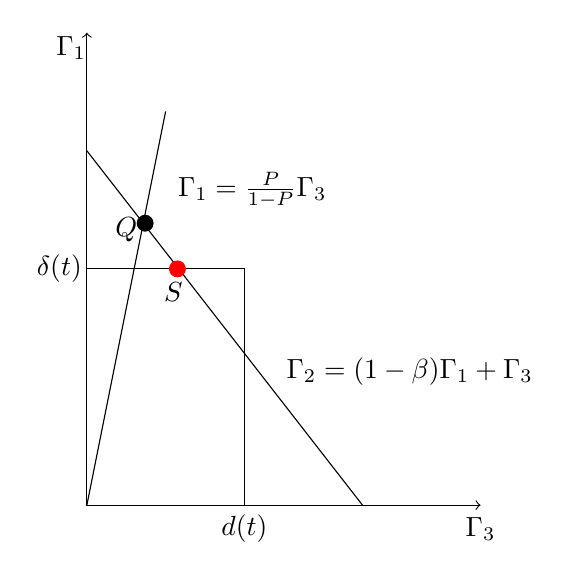
\begin{tikzpicture}
	\draw[<->] (0,6) -- (0,0) --(5,0);
	\draw (0,0) rectangle (2,3);
	\draw (3.5,0) -- (0,4.5);
	\draw (0,0) -- (0.5,2.5) -- (1,5);
	\draw[fill=black](0.74,3.58) circle (0.1);
	\draw[color=red, fill=red](1.15,3) circle (0.1);
	\node (below) at (5,-0.3) {$\Gamma_3$};
	\node (below) at (2,-0.3) {$d(t)$};
	\node (left) at (-0.2,5.8) {$\Gamma_1$};
	\node (left) at (-0.35,3) {$\delta(t)$};
	\node (right) at (4.1,1.7) {$\Gamma_2=(1-\beta)\Gamma_1 +\Gamma_3$};
	\node (right) at (2.1,4) {$\Gamma_1=\frac{P}{1-P}\Gamma_3$};
	\node (left) at (0.5,3.5) {$Q$};
	\node (below) at (1.1,2.7) {$S$};
\end{tikzpicture}